%%%%%%%%%%%%%%%%%%%%%%%%%%%%%%%%%%%%%%%%%
% Article EcoFoG
% Version 2.1 (23/10/2017)
%
% adapté de :
% Stylish Article
% LaTeX Template
% Version 1.0 (31/1/13)
%
% This template has been downloaded from:
% http://www.LaTeXTemplates.com
%
% Original author:
% Mathias Legrand (legrand.mathias@gmail.com)
%
% License:
% CC BY-NC-SA 3.0 (http://creativecommons.org/licenses/by-nc-sa/3.0/)
%
%%%%%%%%%%%%%%%%%%%%%%%%%%%%%%%%%%%%%%%%%


%----------------------------------------------------------------------------------------
%	PACKAGES AND OTHER DOCUMENT CONFIGURATIONS
%----------------------------------------------------------------------------------------

\documentclass[fleqn,10pt]{ArtEcoFoG} % Document font size and equations flushed left

\setcounter{tocdepth}{3} % Show only three levels in the table of contents section: sections, subsections and subsubsections


% Pandoc environments
\usepackage{framed}
\usepackage{fancyvrb}
\providecommand{\tightlist}{%
  \setlength{\itemsep}{0pt}\setlength{\parskip}{0pt}}
\newcommand{\VerbBar}{|}
\newcommand{\VERB}{\Verb[commandchars=\\\{\}]}
\DefineVerbatimEnvironment{Highlighting}{Verbatim}{commandchars=\\\{\}, fontsize=\scriptsize} % Code R
\definecolor{shadecolor}{RGB}{248,248,248}
\newenvironment{Shaded}{\begin{snugshade}}{\end{snugshade}}
\newcommand{\KeywordTok}[1]{\textcolor[rgb]{0.13,0.29,0.53}{\textbf{{#1}}}}
\newcommand{\DataTypeTok}[1]{\textcolor[rgb]{0.13,0.29,0.53}{{#1}}}
\newcommand{\DecValTok}[1]{\textcolor[rgb]{0.00,0.00,0.81}{{#1}}}
\newcommand{\BaseNTok}[1]{\textcolor[rgb]{0.00,0.00,0.81}{{#1}}}
\newcommand{\FloatTok}[1]{\textcolor[rgb]{0.00,0.00,0.81}{{#1}}}
\newcommand{\ConstantTok}[1]{\textcolor[rgb]{0.00,0.00,0.00}{{#1}}}
\newcommand{\CharTok}[1]{\textcolor[rgb]{0.31,0.60,0.02}{{#1}}}
\newcommand{\SpecialCharTok}[1]{\textcolor[rgb]{0.00,0.00,0.00}{{#1}}}
\newcommand{\StringTok}[1]{\textcolor[rgb]{0.31,0.60,0.02}{{#1}}}
\newcommand{\VerbatimStringTok}[1]{\textcolor[rgb]{0.31,0.60,0.02}{{#1}}}
\newcommand{\SpecialStringTok}[1]{\textcolor[rgb]{0.31,0.60,0.02}{{#1}}}
\newcommand{\ImportTok}[1]{{#1}}
\newcommand{\CommentTok}[1]{\textcolor[rgb]{0.56,0.35,0.01}{\textit{{#1}}}}
\newcommand{\DocumentationTok}[1]{\textcolor[rgb]{0.56,0.35,0.01}{\textbf{\textit{{#1}}}}}
\newcommand{\AnnotationTok}[1]{\textcolor[rgb]{0.56,0.35,0.01}{\textbf{\textit{{#1}}}}}
\newcommand{\CommentVarTok}[1]{\textcolor[rgb]{0.56,0.35,0.01}{\textbf{\textit{{#1}}}}}
\newcommand{\OtherTok}[1]{\textcolor[rgb]{0.56,0.35,0.01}{{#1}}}
\newcommand{\FunctionTok}[1]{\textcolor[rgb]{0.00,0.00,0.00}{{#1}}}
\newcommand{\VariableTok}[1]{\textcolor[rgb]{0.00,0.00,0.00}{{#1}}}
\newcommand{\ControlFlowTok}[1]{\textcolor[rgb]{0.13,0.29,0.53}{\textbf{{#1}}}}
\newcommand{\OperatorTok}[1]{\textcolor[rgb]{0.81,0.36,0.00}{\textbf{{#1}}}}
\newcommand{\BuiltInTok}[1]{{#1}}
\newcommand{\ExtensionTok}[1]{{#1}}
\newcommand{\PreprocessorTok}[1]{\textcolor[rgb]{0.56,0.35,0.01}{\textit{{#1}}}}
\newcommand{\AttributeTok}[1]{\textcolor[rgb]{0.77,0.63,0.00}{{#1}}}
\newcommand{\RegionMarkerTok}[1]{{#1}}
\newcommand{\InformationTok}[1]{\textcolor[rgb]{0.56,0.35,0.01}{\textbf{\textit{{#1}}}}}
\newcommand{\WarningTok}[1]{\textcolor[rgb]{0.56,0.35,0.01}{\textbf{\textit{{#1}}}}}
\newcommand{\AlertTok}[1]{\textcolor[rgb]{0.94,0.16,0.16}{{#1}}}
\newcommand{\ErrorTok}[1]{\textcolor[rgb]{0.64,0.00,0.00}{\textbf{{#1}}}}
\newcommand{\NormalTok}[1]{{#1}}
\usepackage{longtable,booktabs}
\usepackage{caption}
% These lines are needed to make table captions work with longtable:
\makeatletter
\def\fnum@table{\tablename~\thetable}
\makeatother
% longtable 2 columns
% https://tex.stackexchange.com/questions/161431/how-to-solve-longtable-is-not-in-1-column-mode-error
\makeatletter
\let\oldlt\longtable
\let\endoldlt\endlongtable
\def\longtable{\@ifnextchar[\longtable@i \longtable@ii}
\def\longtable@i[#1]{\begin{figure}[t]
\onecolumn
\begin{minipage}{0.5\textwidth}\scriptsize
\oldlt[#1]
}
\def\longtable@ii{\begin{figure}[t]
\onecolumn
\begin{minipage}{0.5\textwidth}\scriptsize
\oldlt
}
\def\endlongtable{\endoldlt
\end{minipage}
\twocolumn
\end{figure}}
\makeatother

\usepackage{graphicx,grffile}
\makeatletter
\def\maxwidth{\ifdim\Gin@nat@width>\linewidth\linewidth\else\Gin@nat@width\fi}
\def\maxheight{\ifdim\Gin@nat@height>\textheight0.8\textheight\else\Gin@nat@height\fi}
\makeatother
% Scale images if necessary, so that they will not overflow the page
% margins by default, and it is still possible to overwrite the defaults
% using explicit options in \includegraphics[width, height, ...]{}
\setkeys{Gin}{width=\maxwidth,height=\maxheight,keepaspectratio}

% User-adder preamble
\newlength{\bibitemsep}\setlength{\bibitemsep}{.4\baselineskip}
\newlength{\bibparskip}\setlength{\bibparskip}{0pt}
\let\oldthebibliography\thebibliography \renewcommand\thebibliography[1]{%
  \oldthebibliography{#1}%
  \setlength{\parskip}{\bibitemsep}%
  \setlength{\itemsep}{\bibparskip}%
}

%----------------------------------------------------------------------------------------
%	ARTICLE INFORMATION
%----------------------------------------------------------------------------------------

\JournalInfo{Journées de Rochebrune 2018} % Journal information
\Archive{} % Additional notes (e.g. copyright, DOI, review/research article)

\PaperTitle{Mesure de la biodiversité et de la structuration spatiale de l'activité
économique par l'entropie} % Article title

\Authors{
Eric Marcon\textsuperscript{1*}
} % Authors
\affiliation{
\textsuperscript{1}UMR EcoFoG, AgroParistech, CNRS, Cirad, INRA, Université des Antilles,
Université de Guyane.\\ \hspace{1em} Campus Agronomique, 97310 Kourou, France.
}
\affiliation{*\textbf{Contact}: eric.marcon@ecofog.gf, http://www.ecofog.gf/spip.php?article47} % Corresponding author

\Keywords{entropie, nombres de Hill, diversité, ubiquité, concentration, spécialisation} % Keywords - if you don't want any simply remove all the text between the curly brackets
\newcommand{\keywordname}{Mots-clés} % Defines the keywords heading name

%----------------------------------------------------------------------------------------
%	ABSTRACT
%----------------------------------------------------------------------------------------

\Abstract{
Les mesures de la concentration spatiale et de la spécialisation en
économie sont très similaires à celles de la biodiversité et de
l'ubiquité des espèces en écologie. Les développements méthodologiques
sont plus avancés en écologie, ce qui motive ce travail de transfert
interdisciplinaire. L'entropie est la notion fondamentale, issue de la
physique statistique et la théorie de l'information, utilisée pour
mesurer la concentration et la spécialisation. La notion de nombre
effectif, qui est un nombre de catégories dans une distribution idéale
simplifiée, est introduite. La décomposition de la diversité totale
d'une distribution (la localisation globale en économie) en
concentration ou spécialisation absolue et relative et en redondance,
est présentée. L'ensemble fournit un cadre théorique complet et robuste
pour mesurer la structuration spatiale en espace discret.
}

%----------------------------------------------------------------------------------------

\begin{document}

\selectlanguage{french}

\flushbottom % Makes all text pages the same height

\maketitle % Print the title and abstract box

\tableofcontents % Print the contents section

\thispagestyle{empty} % Removes page numbering from the first page

%----------------------------------------------------------------------------------------
%	ARTICLE CONTENTS
%----------------------------------------------------------------------------------------


\section{Introduction}\label{introduction}

Les recherches sur la structure spatiale de l'activité économique se
sont principalement intéressées à la concentration spatiale, source
d'externalités positives \citep{Marshall1890, Weber1909, Krugman1991},
qui va de pair avec la spécialisation
\citep{Houdebine1999, Cutrini2010}. De nombreuses mesures de
concentration spatiale applicables aux données discrètes \citep[par
opposition aux mesures en espace continu:][]{Marcon2012c} ont été
développées \citep[pour une revue, voir par exemple][]{Combes2015} mais
un cadre méthodologique complet reliant concentration, spécialisation et
mesures d'inégalité en général fait défaut, bien qu'il ait été ébauché
plusieurs fois \citep{Brulhart2005, Mori2005, Cutrini2010}.

Parallèlement, la mesure de la diversité biologique devenue biodiversité
\citep{Wilson1988} et, dans une moindre mesure, de l'ubiquité des
espèces \citep{Levins1968} ont fait l'objet d'une abondante littérature
en écologie statistique \citep[ etc]{Pielou1975, Magurran1988}. Elle
s'est largement inspirée de la théorie de l'information
\citep{Shannon1948} et de la physique statistique \citep{Dewar2008}. Les
mesures de diversité fondées sur l'entropie constituent l'état de l'art
en écologie \citep{Marcon2014d}.

En économie, \citet{Theil1967} a proposé des mesures d'inégalité et de
concentration spatiale similaires à l'entropie de Shannon, mais les
avancées méthodologiques ultérieures sont restées en retrait de celles
de la mesure de la biodiversité. L'objectif de cet article est de
transférer à la discipline de l'économie géographique les derniers
développements de la mesure de la biodiversité pour compléter ses
définitions de la concentration spatiale et de la spécialisation. Les
emprunts très nombreux de méthodes entre disciplines éloignées seront
soulignés.

L'entropie et ses propriétés seront présentées dans la section suivante.
L'application de ces méthodes à la mesure de la concentration spatiale
et de la spécialisation suivront, avant une dernière section de synthèse
consacrée à la localisation globale.

\section{Méthodes}\label{methodes}

\subsection{Questions similaires et notions
opposées}\label{questions-similaires-et-notions-opposees}

Les méthodes présentées ici ont été développées par la littérature sur
la biodiversité. Les écologues ont besoin de mesurer la \emph{diversité}
d'une communauté végétale, composée de plusieurs espèces dont les
effectifs sont connus. Une question moins traitée concerne
l'\emph{ubiquité} des espèces, c'est-à-dire pour une espèce donnée la
diversité des environnements dans lesquels elle se trouve. Cette notion
a été formalisée sous le nom de largeur de niche par \citet{Levins1968},
au sens où la niche écologique est l'ensemble des conditions nécessaires
au développement et à la reproduction d'un être vivant. Pour fixer les
idées et sans perte de généralité, les exemples traités ici concerneront
des arbres dans une forêt tropicale. Chaque arbre appartient à une et
une seule espèce, et le nombre d'individus de chaque espèce est connu.
Les arbres ont une taille qui permet de pondérer leur importance: la
mesure classiquement utilisée est la surface terrière, c'est-à-dire la
surface (horizontale) du tronc découpé à 1,30 m de hauteur
\citep{Husch2016}. Les espèces sont situées dans une taxonomie: elles
sont regroupées par genres et les genres par familles. Enfin, la forêt
est divisée géographiquement en parcelles, elles-mêmes en
sous-parcelles.

En économie géographique, la question probablement la plus traitée est
celle de la \emph{concentration spatiale}
\citep{Ottaviano1998, Combes2015}, source d'externalités positives
\citep{Baldwin2004}. Elle est très semblable à l'ubiquité des espèces
des écologues, mais opposée: une forte concentration est synonyme d'une
faible ubiquité. La \emph{spécialisation} \citep{Amiti1997} est de même
la notion inverse de la diversité. Les exemples traités ici en économie
concerneront les établissements industriels des pays d'Europe fournis
par la base EuroStat en accès libre. Les établissements ont un nombre
d'employés, qui permet leur pondération. Ils appartiennent à un secteur
d'activité, ici selon la nomenclature NUTS, qui est une taxonomie
similaire à celle des espèces biologiques, et leur localisation par pays
peut être détaillée par régions (selon la nomenclature NACE) et leurs
subdivisions.

La spécialisation et la concentration spatiale \citep{Cutrini2010},
comme la diversité et l'ubiquité \citep{Gregorius2010} sont
mathématiquement liées: l'existence de secteurs très concentrés implique
celle de régions spécialisées dans ce secteur. Une approche synthétique
peut être développée: \citet{Cutrini2010} définit la \og localisation
globale\fg{} à cet effet, qui sera généralisée.

\subsection{Données et notations}\label{donnees-et-notations}

Les données ont été choisies pour leur accessibilité et leur simplicité:
il s'agit ici de présenter des méthodes plus que de traiter en détail
des questions économiques complexes. Les applications s'appuieront sur
les nombres de personnes employées par secteur industriel dans 25 pays
européens en 2015. Les données sont disponibles en ligne sur la base
EuroStat \footnote{http://ec.europa.eu/eurostat/web/regions/data/database},
dans le fichier \emph{SBS data by NUTS 2 regions and NACE Rev.~2}.

La nomenclature des secteurs économiques est la NACE (Nomenclature
statistique des Activités économiques dans les Communautés Européennes)
dans sa révision 2. Seuls les secteurs industriels (code NACE : C) ont
été retenus. Les secteurs C12 (manufacture de produits du tabac), C19
(manufacture de coke et produits du pétrole raffiné), C21 (Manufacture
de produits pharmaceutiques de base et préparations pharmaceutiques) et
C30 (Manufacture d'autres équipements de transport) ont été retirés
parce qu'ils présentaient des données manquantes dans des pays majeurs
(par exemple, C30 en Belgique).

Parmi les 30 pays disponibles, Chypre, Malte, l'Irlande, le Luxembourg
et la Slovénie ont été retirés parce qu'ils comportaient trop de données
manquantes. La sélection des données se résume donc à un compromis pour
conserver l'essentiel de l'information, tout à fait discutable mais
suffisant pour les besoins de démonstration méthodologique de cet
article.

Après filtrage, les données se présentent donc sous la forme d'une table
(appelée tableau de contingence) dont les 19 lignes sont les secteurs
industriels et les 25 colonnes les pays retenus. Chaque cellule du
tableau contient le nombre de personnes employées dans le secteur et le
pays considéré, sans données manquantes.

Les secteurs sont indicés par la lettre \(s\) et les pays par la lettre
\(i\). Les effectifs par secteur et pays sont notés \(n_{s,i}\). Les
valeurs marginales sont notées \(n_i\) (l'effectif du pays \(i\), tous
secteurs confondus) et \(n_s\) (celui du secteur \(s\), tous pays
confondus). Pour alléger l'écriture, le niveau d'agrégation
correspondant à l'ensemble des secteurs sera appelé \og l'industrie\fg{}
et celui correspondant à l'ensemble des pays \og l'Europe\fg{}: \(n_s\)
sera donc appelé le nombre de personnes travaillant dans le secteur
\(s\) en Europe. L'effectif total est \(n=\sum_s{n_s}=\sum_i{n_i}\),
égal à 27 419 407. Les tailles relatives des pays et des secteurs sont
représentées en annexe. La probabilité qu'une personne choisie au hasard
travaille dans le secteur \(s\) et le pays \(i\) est notée \(p_{s,i}\)
et estimée par sa fréquence observée \(p_{s,i}=n_{s,i}/n\) (pour alléger
la notation, la fréquence empirique est notée comme la probabilité
théorique plutôt que \(\hat{p}_{s,i}\)). Enfin, les probabilités seront
aussi considérées par secteur ou par région: \(p_{s|i}= p_{s,i}/p_i\)
est la probabilité pour une personne du pays \(i\) de travailler dans le
secteur \(s\) dont la somme sur tous les secteurs vaut 1
(\(\sum_s{p_{s|i}}=1\)). Le vecteur des probabilités \(p_{s|i}\) de tous
les secteurs dans le pays \(i\) est noté \(\mathbf{p_{s|i}}\). De même,
\(p_{i|s}\) est la probabilité, dans le secteur \(s\) choisi, qu'une
personne travaille dans le pays \(i\) et \(\mathbf{p_{i|s}}\) est le
vecteur des probabilité des pays pour le secteur \(s\). Enfin, les
probabilités marginales sont notées \(p_s\) et \(p_i\); elles sont
estimées respectivement par \(n_{s}/n\) et \(n_{i}/n\).

Les données et le code R \citep{R} nécessaires pour reproduire
l'intégralité des résultats se trouvent en annexe. Le code utilise
largement le package \emph{entropart} \citep{Marcon2014c} consacré à la
mesure de la biodiversité.

\subsection{L'entropie comme mesure
d'incertitude}\label{lentropie-comme-mesure-dincertitude}

Les notions étant établies, il s'agit maintenant de les traduire en
mesures opérationnelles permettant de comparer la diversité de
différentes communautés végétales ou la spécialisation de régions
industrielles, de donner un sens concret, facilement compréhensible, à
ces mesures, et de caractériser leurs propriétés pour pouvoir les
utiliser par exemple dans le cadre de modèles.

La diversité biologique est un déterminant important du fonctionnement
des écosystèmes \citep{Chapin2000}. Parmi de très nombreuses mesures
\emph{ad-hoc} développées selon les besoins \citep{Peet1974}, l'intérêt
de l'entropie de \citet{Shannon1948} a été argumenté notamment par
\citet{Pielou1975} dans un ouvrage de référence. En économétrie, les
travaux de \citet{Davis1941} et surtout \citet{Theil1967} ont ouvert la
voie. Le très connu indice de Theil est la différence entre l'entropie
de Shannon et sa valeur maximale possible, ce qui illustre l'opposition
des approches présentée plus haut en même temps que la convergence des
méthodes.

L'entropie est, entre autres, une mesure d'incertitude qu'il est temps
de formaliser. Définissons une expérience (par exemple l'échantillonnage
d'un arbre au hasard dans une forêt) dont l'ensemble des résultats
possibles (l'espèce à laquelle il appartient) est connu. Les résultats
sont notés \(r_s\) où l'indice \(s\) prend toutes les valeurs possibles
entre 1 et \(S\), le nombre de résultats possibles. La probabilité
d'obtenir \(r_s\) est \(p_s\), et \(\mathbf{p_s}=(p_1,p_2,\dots,p_S)\)
est l'ensemble (mathématiquement, le vecteur) des probabilités d'obtenir
chaque résultat. L'obtention du résultat \(r_s\) est peu étonnante si
\(p_s\) est grande: elle apporte peu d'information supplémentaire par
rapport à la simple connaissance des probabilités. En revanche, si
l'espèce \(r_s\) est rare (\(p_s\) est petite), son tirage est
surprenant. La notion d'information, définie par Shannon, est identique
à celle de surprise, plus intuitive. On définit donc une fonction
d'information, \(I(p_s)\), décroissante quand la probabilité augmente,
de \(I(0)=+\infty\) (ou éventuellement une valeur strictement positive
finie) à \(I(1)=0\) (l'observation d'un résultat certain n'apporte
aucune surprise).

L'entropie est définie comme la moyenne de l'information apportée par
tous les résultats possibles de l'expérience. Comme chaque résultat à la
probabilité \(p_s\) d'être réalisée, la moyenne sur tous les résultats
possibles est la moyenne pondérée de \(I(p_s)\). L'entropie est définie
comme \[H(\mathbf{p_s})=\sum_{s}{p_s I(p_s)}.\]

\subsubsection{Entropie de Shannon}\label{entropie-de-shannon}

Shannon a utilisé la fonction d'information \(I(p_s)=-\ln{p_s}\) pour
ses propriétés mathématiques. Elle peut être écrite sous la forme
\(I(p_s)=\ln({1/p_s})\). L'inverse de la probabilité, \(1/p_s\), sera
appelé \emph{rareté}: une espèce très rare a une probabilité proche de
0. La fonction d'information utilisée par Shannon est donc le logarithme
de la rareté.

Le terme \og entropie\fg{} avait été introduit par Clausius en 1865 pour
sa nouvelle formulation du second principe de la thermodynamique énoncé
par Carnot 40 ans plus tôt. Son étymologie grecque signifie
\emph{transformation} parce que le second principe concerne la variation
d'entropie. Boltzmann a caractérisé l'entropie d'un système complexe (un
gaz, donc chaque particule peut avoir plusieurs états possibles) en
1877. \citet{Shannon1948} a enfin montré que le nombre d'états possibles
d'un système est analogue au nombre de messages d'une longueur choisie
pouvant être créés en assemblant les lettres d'un alphabet dont les
fréquences des lettres sont fixées. L'entropie de Shannon est, à une
constante près, égale à celle de Boltzmann normalisée par la longueur du
message, dont elle est indépendante. Cette propriété fondamentale lui
permet de décrire la complexité d'un système non seulement par le nombre
possible de ses états, mais plus simplement par la fréquence relative de
ses composants, donnant naissance à la théorie de l'information.

La pertinence de l'entropie comme mesure de diversité en découle
directement: un système est d'autant plus divers qu'il peut avoir un
grand nombre d'état possibles ou, de manière équivalente, qu'il est
difficile de prévoir l'état dans lequel il se trouve, ou encore qu'il a
une entropie élevée.

\subsubsection{Entropie généralisée}\label{entropie-generalisee}

De nombreuses fonctions d'informations alternatives sont envisageables,
y compris les plus exotiques comme \(I(p_s)=\cos({p_s \pi/2})\)
\citep{Gregorius2014}.

Parmi elles, trois familles de fonctions paramétrisables se sont
imposées : l'entropie généralisée de la littérature des inégalités
\citep{Shorrocks1980}, l'entropie de \citet{Renyi1961}, très utilisée
jusqu'aux années 2000 pour la mesure de la biodiversité et, plus
récemment, l'entropie HCDT détaillée ici.

\citet{Tsallis1988} a proposé une cette entropie généralisée en physique
statistique pour des systèmes ne répondant pas aux propriétés
nécessaires à la théorie de Boltzmann. Elle avait été définie par
\citet{Havrda1967} en cybernétique et redécouverte ensuite, notamment
par \citet{Daroczy1970} en théorie de l'information, d'où son nom,
entropie \emph{HCDT} (voir \citet{Mendes2008}, page 451, pour un
historique complet).

Sa forme mathématique est:
\[ ^{q}H(\mathbf{p_s}) = \frac{1}{q-1}\left(1-\sum^S_{s=1}{p^q_s}\right),\]
où \(q\) est un paramètre arbitraire. \(^{1}H\) n'est pas définie
directement mais on montre que \(^{q}H\) tend vers l'entropie de Shannon
quand \(q \to 1\).

Son intérêt apparaît plus clairement en définissant une généralisation
de la fonction logarithme, le logarithme déformé d'ordre \(q\)
\citep{Tsallis1994} comme \[\ln_q{x} = \frac{x^{1-q}-1}{1-q}.\] Ici
encore, \(\ln_q{x}\) tend vers le logarithme naturel quand \(q\) tend
vers 1. L'entropie HCDT s'écrit alors comme une généralisation de
l'entropie de Shannon :
\[^{q}H(\mathbf{p_s}) = \sum_{s}{p_s \ln_q{(1/p_s)}}\]

Le logarithme déformé est une fonction qui, comme son nom l'indique,
déforme la fonction logarithme naturel en changeant sa courbure mais en
respectant, quel que soit \(q\), \(\ln_q{1}=0\) et les limites
(\(-\infty\) quand \(x \to 0\) et \(+\infty\) quand \(x \to \infty\)).
En faisant varier le paramètre \(q\), la fonction d'information
\(\ln_q{(1/p_s)}\) attribue une plus grande (quand q, supérieur à 1,
croît) ou moins grande (quand q, inférieur à 1, décroît) surprise aux
espèces rares (dont la rareté, \(1/p_s\), est grande).

On dispose à ce stade d'une définition simple et générale : l'entropie
(d'ordre \(q\)) d'un système est la surprise moyenne apportée par
l'observation d'un de ses individus; la surprise est le logarithme
(d'ordre \(q\)) de la rareté. Une communauté biologique est d'autant
plus diverse qu'elle est surprenante (que son entropie est grande). Une
région est d'autant plus spécialisée que son entropie est faible.

Trois valeurs de \(q\) sont particulièrement intéressantes:

\begin{itemize}
\item
  \(q=0\): l'entropie est la richesse, c'est-à-dire \(S\), le nombre
  d'espèces ou de secteurs, moins 1 ;
\item
  \(q=1\): l'entropie est celle de Shannon. En économétrie, \(S-^{1}H\)
  est l'indice de Theil;
\item
  \(q=2\): l'entropie est l'indice de biodiversité de
  \citet{Simpson1949}, c'est-à-dire la probabilité que deux individus
  choisis au hasard appartiennent à une espèce différente. En
  économétrie, son complément à 1, c'est à dire la probabilité que deux
  individus appartiennent au même secteur, est l'indice de Herfindahl,
  ou Herfindahl-Hirschman \citep{Hirschman1964}, qui mesure ici la
  spécialisation.
\end{itemize}

Les valeurs négatives de \(q\) donnent à une espèce une importance
d'autant plus grande qu'elle est rare alors qu'à \(q=0\) toutes les
espèces contribuent de façon identique à l'entropie (elles sont
simplement comptées, quelle que soit leur probabilité). Leur intérêt est
donc limité. Comme leurs propriétés mathématiques sont mauvaises
\citep{Marcon2014a}, elles ne sont en pratique pas utilisées. Les
valeurs de \(q\) supérieures à 2 sont peu utilisées parce qu'elles
négligent trop les espèces qui ne sont pas les plus fréquentes.

\subsubsection{De l'entropie à la
diversité}\label{de-lentropie-a-la-diversite}

L'entropie a un sens physique : c'est une quantité de surprise; c'est
donc bien plus qu'un indice, qui n'est qu'une valeur arbitraire devant
seulement respecter une relation d'ordre pour permettre des
comparaisons. Cependant, à l'exception des ordres 0 et 2, la valeur de
l'entropie n'a pas d'interprétation intuitive. Les nombres de Hill
répondent à ce manque.

Le souhait de \citet{Hill1973} était de rendre les indices de diversité
intelligibles après l'article remarqué de \citet{Hurlbert1971} intitulé
\og le non-concept de diversité spécifique\fg{}. Hurlbert reprochait à
la littérature sur la diversité sa trop grande abstraction et son
éloignement des réalités biologiques, notamment en fournissant des
exemples dans lesquels l'ordre des communautés n'était pas le même selon
l'indice de diversité choisi.

Les nombres de Hill sont le nombre d'espèces équiprobables donnant la
même valeur d'entropie que la distribution observée, autrement dit des
\emph{nombres effectifs} d'espèces, encore appelés \emph{nombres
équivalents}. Le concept a été défini rigoureusement par
\citet{Gregorius1991}, d'après \citet{Wright1931} qui avait le premier
défini la taille effective d'une population en génétique: étant donné
une variable caractéristique (ici, l'entropie) fonction seulement d'une
variable numérique (ici, le nombre d'espèces) dans un cas idéal (ici,
l'équiprobabilité des espèces), le nombre effectif est la valeur de la
variable numérique pour laquelle la variable caractéristique est celle
du jeu de données.

Formellement, ils sont simplement l'exponentielle déformée de l'entropie
HCDT \citep{Marcon2014a}. La fonction exponentielle déformée d'ordre
\(q\) est la fonction réciproque du logarithme déformé, dont la valeur
est \[e^x_q = [1 + (1-q)x]^{1/(1-q)}.\]

Le nombre de Hill d'ordre \(q\), appelé simplement \emph{diversité
d'ordre \(q\)} \citep{Jost2006} est donc
\[^{q}D(\mathbf{p_s}) = e_q^{^{q}H(\mathbf{p_s})}.\]

La formulation explicite à partir des probabilités est:
\[^{q}D(\mathbf{p_s}) = \left( \sum_{s}{p^q_s} \right)^{1/(1-q)}.\] Ces
résultats avaient déjà été obtenus avec une autre approche par
\citet{MacArthur1965} et repris par \citet{Adelman1969} dans la
littérature économique. Aussi, la mesure d'inégalité
d'\citet{Atkinson1970} est très similaire aux nombres de Hill.

\subsubsection{Profils de diversité}\label{profils-de-diversite}

La diversité étant exprimée dans la même unité (un nombre d'espèces)
quel que soit son ordre, il est possible de tracer un profil de
diversité, c'est-à-dire la valeur de \(^{q}D\) en fonction de \(q\). Les
courbes de deux communautés peuvent se croiser parce que le poids des
espèces rares diminue avec l'augmentation de \(q\). Si ce n'est pas le
cas, la relation d'ordre entre les communautés est bien définie
\citep{Tothmeresz1995}.

\subsection{La décomposition de
l'entropie}\label{la-decomposition-de-lentropie}

La notion de diversité \(\beta\) a été introduite par
\citet{Whittaker1960} comme le degré de différenciation des communautés
biologiques. La question traitée est celle de la décomposition de la
diversité de données agrégées (la diversité des secteurs économiques en
Europe) à un niveau plus détaillé (par pays). La diversité du niveau le
plus agrégé a été appelée \(\gamma\) par Whittaker, la diversité moyenne
des niveaux détaillés \(\alpha\), et la différenciation entre les
niveaux détaillés \(\beta\). Il est évident que les diversités
\(\gamma\) et \(\alpha\) sont de même nature, seul le niveau de détail
des données diffère. En revanche, la caractérisation de la diversité
\(\beta\) a généré des controverses \citep{Ellison2010a}.

En économie, la décomposition des mesures d'inégalité a suivi une voie
parallèle à celle des écologues \citep{Bourguignon1979}. Celle de la
concentration spatiale est restée limitée à l'entropie de Theil
\citep{Mori2005, Cutrini2010} à l'exception notable de
\citet{Brulhart2005} qui ont utilisé l'entropie généralisée de
\citet{Shorrocks1980}.

\citet{Jost2007} a montré que la décomposition de l'entropie est
additive : l'entropie \(\beta\) est la différence entre les entropies
\(\gamma\) et \(\alpha\). \citet{Marcon2012a} ont ensuite interprété
l'entropie \(\beta\) comme l'information supplémentaire apportée par la
connaissance des distributions désagrégées en plus de celle des données
agrégées, c'est-à-dire une entropie relative. Cette information est la
divergence entre les distributions, c'est-à-dire une mesure mathématique
de l'écart entre leurs valeurs. La divergence de \citet{Kullback1951}
est bien connue des économistes sous le nom d'entropie relative de Theil
\citep{Conceicao2000}. La différence entre l'entropie \(\gamma\) d'ordre
1 et la moyenne des entropies d'ordre 1 des distributions désagrégées
est la moyenne des divergences de Kullback-Leibler correspondantes,
appelée par les physiciens statistiques \og divergence de
Jensen-Shannon\fg{}. \citet{Marcon2014a} ont généralisé ce résultat à
tous les ordres de l'entropie HCDT.

Comme l'entropie \(\gamma\) et \(\alpha\), l'entropie \(\beta\) peut
être transformée en un nombre effectif qui est le nombre de communautés
de même poids, sans espèce commune, qui auraient la même entropie
\(\beta\) que les communautés réelles. La décomposition de la diversité
est multiplicative : la diversité \(\gamma\) est le produit des
diversités \(\alpha\) et \(\beta\).

La décomposition complète est finalement un produit de nombres effectifs
: la diversité de l'assemblage de plusieurs communautés biologiques,
appelée diversité \(\gamma\) est un nombre effectif d'espèces; c'est le
produit du nombre effectif d'espèces de chaque communauté (diversité
\(\alpha\)) par le nombre effectif de communautés (diversité \(\beta\)).
Elle sera appliquée dans cet article à l'économie des pays européens :
le nombre effectif de secteurs économiques de l'Europe (\(\gamma\)) est
le produit du nombre effectif moyen de secteurs des pays (\(\alpha\))
par un nombre effectif de pays (\(\beta\)).

De même, l'ubiquité d'un secteur économique aggrégé (l'industrie
manufacturière) est un nombre effectif de pays (\(\gamma\)),
décomposable en un nombre effectif de pays par secteur désagrégé
(\(\alpha\)) multiplié par un nombre effectif de secteurs désagrégés
(\(\beta\)).

La décomposition sera limitée ici à un seul niveau de désagrégation des
données. Elle peut être répétée : les pays peuvent être découpés en
régions, les régions en départements\ldots{} Le nombre effectif de
secteurs économiques de l'Europe (\(\gamma\)) peut alors être décomposé
en un nombre effectif de pays (\(\beta_1\)) fois un nombre effectif de
régions (\(\beta_2\)) fois un nombre effectif de départements
(\(\beta_3\)) fois un nombre effectif de secteurs par département
(\(\alpha\)). La décomposition hiérarchique de la diversité a été
traitée notamment par \citet{Marcon2012a}; \citet{Richard-Hansen2015};
\citet{Pavoine2015a}.

\subsection{Diversité jointe: information mutuelle et
redondance}\label{diversite-jointe-information-mutuelle-et-redondance}

Nous avons vu que l'entropie pouvait être utilisée selon les deux points
de vue de la diversité et de l'ubiquité (de façon équivalente: la
spécialisation et la concentration spatiale). Les données sont les mêmes
et peuvent être représentés dans le tableau de contingence dont les
lignes représentent par exemple les secteurs industriels alors que les
colonnes représentent les pays, chaque cellule de la table fournissant
l'abondance (en nombre d'établissements ou de personnes travaillant)
d'un secteur dans un pays.

La diversité des pays est calculée en traitant chaque colonne du
tableau, l'ubiquité des secteurs en traitant chaque ligne. La diversité
\(^{q}D(\mathbf{p_s})\) de l'Europe entière (l'agrégation des pays) est
obtenue, comme l'ubiquité des secteurs agrégés \(^{q}D(\mathbf{p_i})\),
à partir des des probabilités marginales. La diversité
\(^{q}D(\mathbf{p_{s,i}})\) de l'ensemble des données, tous secteurs et
pays confondus, a un grand intérêt, notamment théorique pour l'entropie
de Shannon \citep{Faddeev1956, Baez2011}: elle est appelée diversité
jointe \citep{Gregorius2010}.

La différence entre l'entropie jointe et la somme des entropies
marginales (celle de l'ensemble des secteurs et celle de l'ensemble des
pays),
\(^{q}H(\mathbf{p_{s,i}})-^{q}H(\mathbf{p_{s}})-^{q}H(\mathbf{p_{i}})\),
s'appelle l'information mutuelle. L'entropie de Shannon (mais pas
l'entropie HCDT d'ordre différent de 1) de deux systèmes indépendants
s'additionne: si l'appartenance aux pays est indépendante de
l'appartenance aux secteurs, c'est-à-dire si la probabilité \(p_{s,i}\)
est simplement le produit des probabilités \(p_{s}\) et \(p_{i}\), alors
l'entropie de Shannon jointe est nulle. En d'autres termes,
l'information mutuelle est l'entropie supplémentaire apportée par la non
indépendance des lignes et des colonnes du tableau. Elle est égale aux
deux entropies \(\beta\), celle de la diversité et celle de l'ubiquité.
Ces propriétés ne sont valables que pour l'entropie de Shannon mais ont
été utilisées sous différentes formes dans la littérature \citep[par
exemple][]{Cutrini2009, Chao2013}.

Quel que soit l'ordre considéré, \citet{Gregorius2010} a montré que la
diversité jointe apporte une information supplémentaire importante sur
la distribution des abondances qui n'est pas prise en compte par la
décomposition de la diversité déjà présentée. L'exemple de la
biodiversité est utilisé ici pour simplifier l'exposé. La diversité
\(\alpha\) est le nombre d'espèces équiprobables dans une communauté
type. La diversité \(\beta\) est le nombre de ces communautés types,
équiprobables et sans espèce commune. La diversité \(\gamma\) est le
produit des deux précédentes, un nombre d'espèces équiprobables
résultant de l'assemblage des communautés. Chaque espèce n'apparaît que
dans une communauté dans cette représentation. La réplication à
l'identique des communautés ne modifie pas les diversités \(\alpha\),
\(\beta\) et \(\gamma\), c'est même une propriété demandée aux mesures
de diversité \citep{Hill1973}. En revanche, la diversité jointe est
multipliée par le nombre de réplications \citep{Marcon2014d}: le rapport
entre la diversité jointe et la diversité \(\beta\) mesure la redondance
sous la forme d'un nombre effectif, le nombre de répétitions des
communautés.

La redondance n'a que peu d'applications pratiques en écologie parce que
les données disponibles sont en général des échantillons des communautés
étudiées (des placettes d'inventaire forestier par exemple). Leur
redondance reflète l'effort d'échantillonnage, qui est un choix de
l'expérimentateur. Lorsque les données sont exhaustives ou, plus
généralement, lorsque les probabilités marginales des communautés sont
interprétables comme leurs tailles, la redondance est une information
aussi importante que la diversité.

\section{Concentration spatiale et
spécialisation}\label{concentration-spatiale-et-specialisation}

Les méthodes présentées jusqu'ici, issues de la physique et de
l'écologie statistiques, ont des applications intéressantes en économie.
Deux questions seront traitées : celle de la mesure de la concentration
spatiale des activités économiques et celle de la décomposition de la
localisation globale.

La concentration spatiale des activités économiques est un sujet
important de la littérature \citep{Combes2015}. La première étape de la
compréhension des phénomènes économiques en jeu est la caractérisation
de la concentration. Une étape majeure a été franchie par
\citet{Ellison1997} qui ont posé clairement le principe d'une mesure
relative (la distribution géographique d'un secteur industriel est
comparée à celle de la taille des régions où elle est considérée,
principe résumé sous le titre d'approche du jeu de fléchettes) et celui
du test statistique de la distribution observée contre sa valeur sous
une hypothèse nulle appropriée : une distribution uniforme et
indépendante. Ces caractéristiques font défaut à des indices de
concentration antérieurs, comme l'indice de Gini
\citep{Gini1912, Ceriani2012} dont la valeur observée ne peut être
comparée qu'à ses extrêmes possibles.

La statistique centrale de l'indice d'Ellison et Glaeser pour le secteur
\(s\) est, avec nos notations, \(G_s=\sum_i{(p_{i|s} - p_i)^2}\),
c'est-à-dire la somme des carrés des écarts entre la part du pays \(i\)
dans l'effectif total du secteur \(s\) et la part du pays \(i\) dans
l'industrie, tous secteurs confondus. En termes mathématiques, \(G\) est
la distance \(L^2\) entre la distribution observée du secteur \(s\) et
sa distribution attendue, celle de l'industrie en général.

L'indice relatif de \citet{Theil1967} est parfois utilisé dans le même
objectif \citep{Cutrini2009}: il mesure aussi l'écart entre la
distribution observée et la distribution attendue, mais avec une autre
métrique : la divergence de Kullback-Leibler.

L'entropie HCDT permet d'unifier et étendre ces approches. La
concentration, absolue puis relative, sera envisagée en premier. La
spécialisation suivra.

\subsection{Concentration spatiale}\label{concentration-spatiale}

\subsubsection{Ubiquité et concentration
absolue}\label{ubiquite-et-concentration-absolue}

L'ubiquité du secteur \(s\), \(^{q}D(\mathbf{p_{i|s}})\) est le nombre
effectif de pays qu'il occupe. L'ubiquité peut être calculée pour
n'importe quel niveau de regroupement sectoriel, ici pour l'industrie
entière (code NACE C) ou par secteur détaillé. Un profil d'ubiquité peut
être tracé pour chaque secteur. Aux faibles ordres, l'ubiquité donne une
grande importance aux pays peu occupés. À \(q=0\), l'ubiquité est
simplement le nombre de pays dans lesquels le secteur est présent. Aux
grands ordres, seuls les pays occupés majoritairement contribuent à
l'ubiquité.

\begin{figure}
\centering
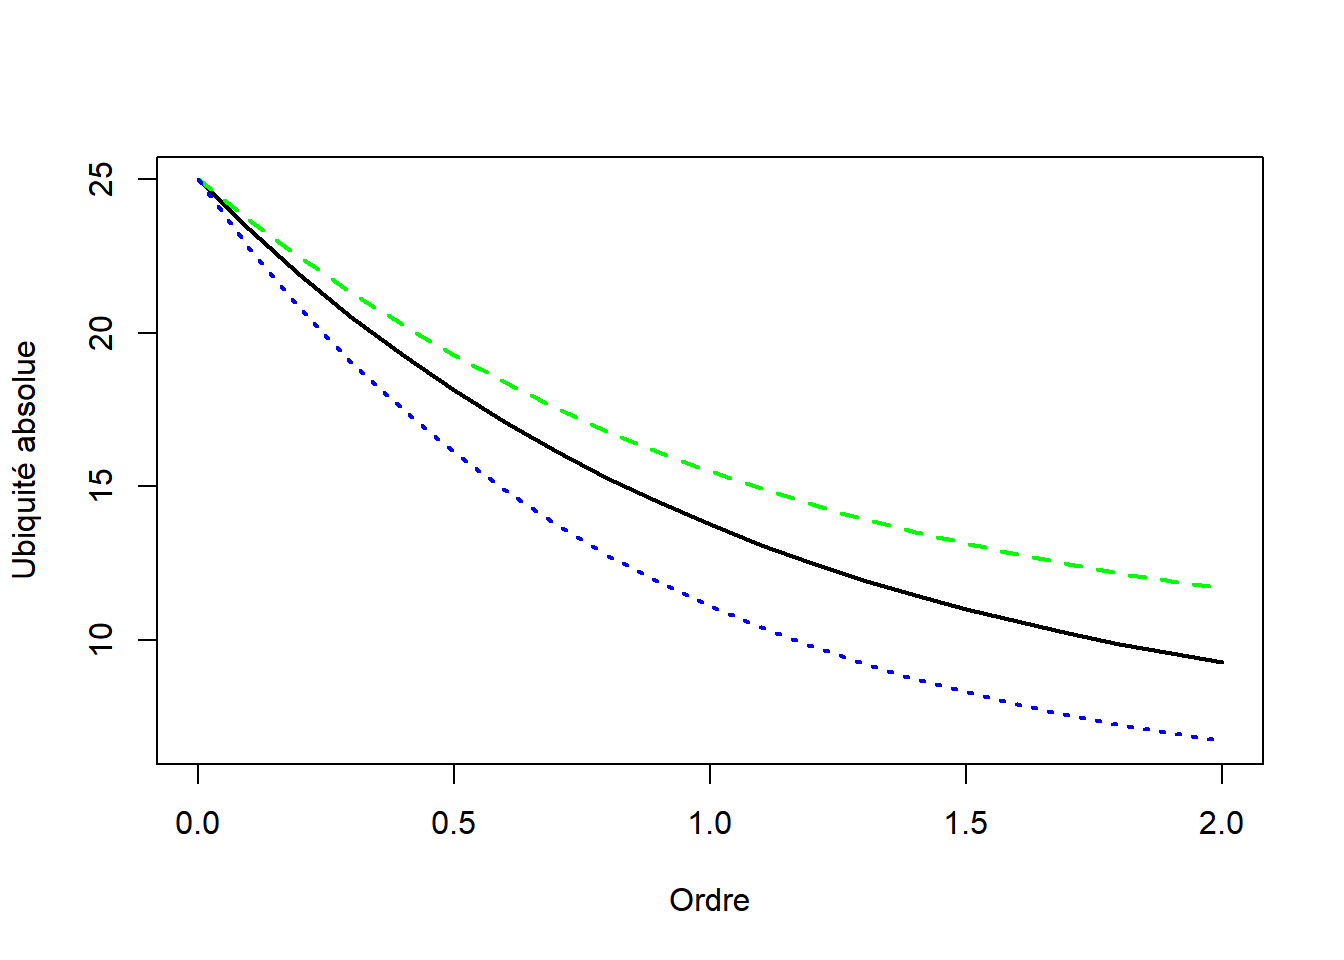
\includegraphics{Entropie_files/figure-latex/uC-1.pdf}
\caption{\label{fig:uC}Profils d'ubiquité absolue de l'industrie (courbe
pleine, noire), du secteur C10 (pointillés longs, verts) et du secteur
C20 (pointillés courts, bleus)}
\end{figure}

La figure \ref{fig:uC} présente les profils d'ubiquité de l'industrie
entière et des secteurs C10 (Manufacture de produits alimentaires) et
C20 (Manufacture de produits chimiques) qui s'écartent le plus, parmi
tous les secteurs étudiés, de l'industrie entière. L'ubiquité est
mesurée en nombre effectifs de pays. Les secteurs sont présents dans
tous les pays (les données sont très agrégées) donc l'ubiquité d'ordre 0
est toujours égale au maximum possible, 25. À l'ordre 2, à l'autre
extrémité des courbes, 9.3 pays occupés par le même nombre de personnes
suffiraient pour obtenir le même niveau d'ubiquité que celui observé
pour l'ensemble de l'industrie.

L'ubiquité est la notion opposée à celle de concentration. Une
transformation simple des valeurs d'ubiquité permet de les traduire en
niveau de concentration plus conformes à la culture économique. Le
complément de l'ubiquité au nombre de pays est une bonne mesure de la
concentration en tant que nombre effectif de pays délaissés par le
secteur étudiés. Il peut être normalisé par le nombre de pays moins 1
pour obtenir une valeur entre 0 et 1 présentée en figure \ref{fig:cC}.

\begin{figure}
\centering
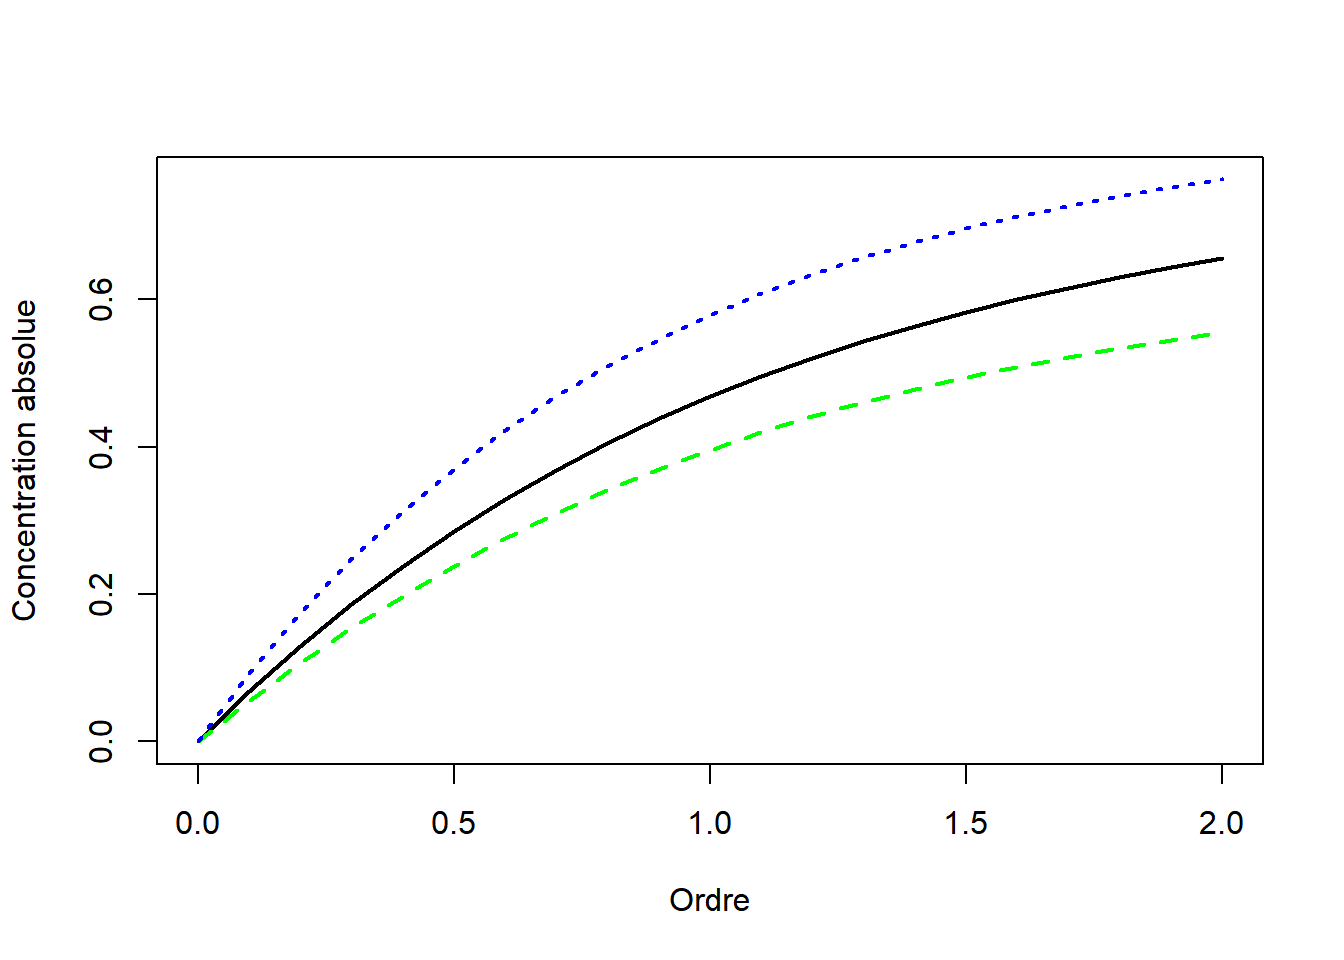
\includegraphics{Entropie_files/figure-latex/cC-1.pdf}
\caption{\label{fig:cC}Profils de concentration absolue de l'industrie
(courbe pleine, noire), du secteur C10 (pointillés longs, verts) et du
secteur C20 (pointillés courts, bleus).}
\end{figure}

La valeur de la concentration est la proportion des pays délaissés (en
nombres effectifs). Une valeur de 0 signifie que tous les pays sont
occupés, une valeur de 1 que tout le secteur est concentré dans un seul
pays. L'industrie chimique, C20, est beaucoup plus concentrée que
l'industrie en général, alors que l'industrie agro-alimentaire, C10,
l'est nettement moins. Ces résultats sont valides à tous les ordres,
sauf près de 0, lorsque la présence seule du secteur compte, quel que
soit son abondance.

Cette mesure de l'ubiquité ou de la concentration est absolue
\citep{Brulhart2005}: elle ne compare le nombre effectif de secteurs à
aucune référence externe. Pour son interprétation, une comparaison à une
autre mesure absolue (la concentration à un niveau plus agrégé) est
nécessaire \citep{Marcon2012c}

\subsubsection{Concentration relative}\label{concentration-relative}

L'ubiquité absolue a été calculée au niveau des secteurs désagrégés (C10
et C20) et au niveau de l'industrie entière, dont les effectifs ont été
obtenus par agrégation des ceux des secteurs. En reprenant la
terminologie de la décomposition de la biodiversité, l'ubiquité absolue
de l'industrie entière est l'ubiquité \(\gamma\), égale au produit de
l'ubiquité \(\alpha\) (la moyenne des de celle des secteurs désagrégés)
par l'ubiquité \(\beta\), nombre effectif de secteurs équiprobables, ne
partageant aucun pays.

La décomposition de l'entropie est la même, mais l'entropie \(\gamma\)
est la somme des entropies \(\alpha\) et \(\beta\). L'entropie \(\beta\)
est, comme on l'a vu, la divergence de Jensen-Shannon généralisée entre
la distribution de chaque secteur et la distribution agrégée de
l'industrie. Aux ordres particuliers \(q=1\) et \(q=2\), cette
divergence est la moyenne, pondérée par les poids des secteurs, de
l'entropie relative de Theil et de la statistique \(G_s\) d'Ellison et
Glaeser. Ces indices classiques de concentration spatiale sont des
divergences de Kullback-Leibler généralisées, en d'autres termes des
entropies \(\beta\) d'ordres particuliers, donnant une importance
différente aux pays à faibles effectifs: l'indice d'Ellison et Glaeser,
d'ordre 2, ne prend en compte que les implantations dominantes.

L'entropie \(\beta\) mesure la concentration relative: elle intègre une
référence (la distribution de l'industrie tous secteurs confondus) et a
donc une valeur attendue, 0, si la distribution de l'industrie
considérée est identique à celle de référence.

Sa valeur n'est pas interprétable intuitivement: il faut recourir à
l'ubiquité \(\beta\), nombre effectif de secteurs dont l'interprétation
est claire. Dans le cadre de la décomposition présenté plus haut,
l'ubiquité \(\beta\), concentration relative moyenne, est le rapport de
l'ubiquité \(\gamma\) sur l'ubiquité \(\alpha\): elle s'applique à
l'ensemble des secteurs mais ne donne pas d'information sur un secteur
particulier. Elle doit donc être détaillée pour chaque secteur : la
concentration relative du secteur \(s\) est définie comme le rapport
entre l'ubiquité absolue de l'ensemble de l'industrie (\(\gamma\)) et
son ubiquité absolue propre:
\[^{q}C_{s} = ^{q}D(\mathbf{p_{i}}) / ^{q}D(\mathbf{p_{i|s}}).\]

C'est un nombre effectif de secteurs: si tous les secteurs avaient une
ubiquité égale au nombre effectif de pays \(^{q}D(\mathbf{p_{i|s}})\),
il en faudrait \(^{q}C_{s}\) pour obtenir une industrie dont l'ubiquité
serait \(^{q}D(\mathbf{p_{i}})\) pays effectifs.

La valeur de la concentration relative est visible sur la figure
\ref{fig:uC}: elle est égale au rapport entre les valeurs des profils
d'ubiquité de l'industrie et du secteur considéré. Pour l'industrie
chimique (C20), elle varie de 1 (à l'ordre 0) à 1.4 à l'ordre 2: 1.4
secteurs effectifs d'ubiquité effective celle du secteur C20, soit 6.7
pays, formeraient une industrie dont l'ubiquité serait celle observée
pour l'industrie européenne, \(6.7 \times 1.4 = 9.3\) pays effectifs.

La concentration est inférieure à 1 pour l'industrie agro-alimentaire
(C20): 0.79 secteurs effectifs de même caractéristiques que le secteur
C10 suffiraient pour constituer l'ubiquité de l'industrie européenne. En
d'autres termes, le secteur C10 est relativement dispersé.

La concentration relative et l'ubiquité absolue (figure \ref{fig:uC})
sont liées : leur produit est la concentration absolue de l'ensemble des
secteurs, prise comme référence. La concentration absolue (figure
\ref{fig:cC}) va donc de pair avec la concentration relative, mais les
informations qu'elles fournissent sont différentes.

Dans la littérature économique, l'entropie relative a été utilisée pour
mesurer la concentration relative par \citet{Brulhart2005}.
\citet{Mori2005} ont utilisé la divergence de Kullback-Leibler entre la
distribution d'un secteur et celle de la surface (au lieu du nombre de
personnes travaillant dans l'industrie) des régions du Japon pour
mesurer la concentration topographique (et non relative) des secteurs.
\citet{Rysman2005} ont proposé un test de la concentration relative d'un
secteur fondé sur le rapport de vraisemblance des distributions du
secteur et de l'industrie entière, qui est simplement la divergence de
Kullback-Leibler \citep[voir][ pour une présentation détaillée des liens
entre les deux approches]{Mori2005}. \citet{Alonso-Villar2013} ont
proposé une décomposition de l'entropie généralisée mais se sont limités
en pratique à l'ordre 1.

L'entropie relative de Theil a été utilisée pour comparer l'évolution de
la concentration spatiale dans le temps \citep[par
exemple,][]{Cutrini2010} puisqu'elle obéit bien à une relation d'ordre
comme toute entropie. Enfin, \citet{Bickenbach2013} ont combiné l'indice
de Theil (absolu) et l'indice relatif de Theil pour mieux décrire la
concentration spatiale en les appliquant à des secteurs économiques
différents (industrie et services).

\subsection{Spécialisation}\label{specialisation}

\begin{figure}
\centering
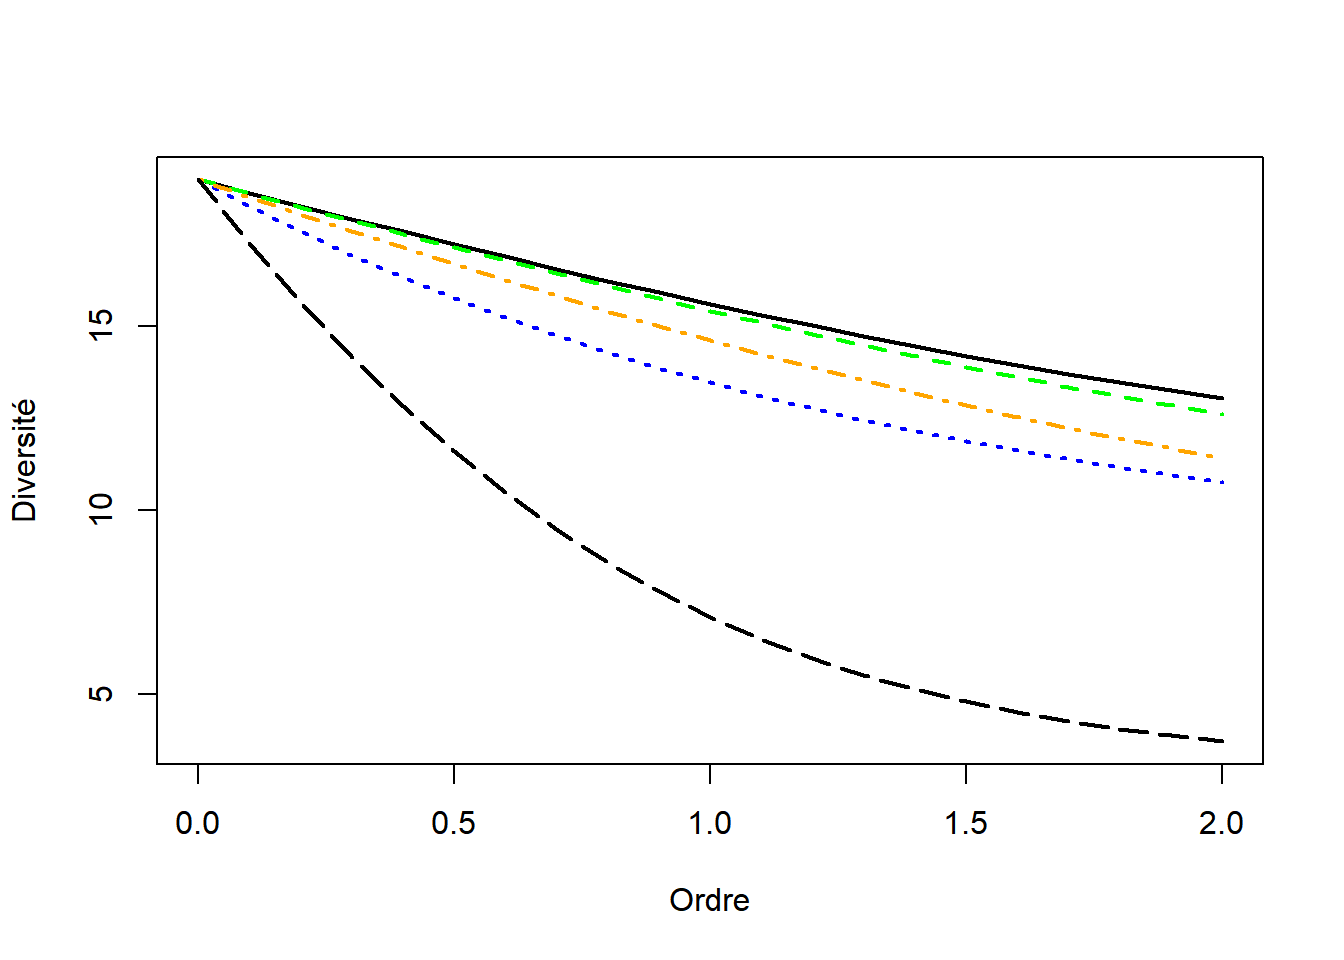
\includegraphics{Entropie_files/figure-latex/d-1.pdf}
\caption{\label{fig:d}Profils de diversité de l'Europe (courbe pleine,
noire), de l'Italie (pointillés longs, verts), de la France (pointillés
alternés, orange), de l'Allemagne (pointillés courts, bleus) et de
l'Islande (pointillés très longs, noirs).}
\end{figure}

La mesure de la spécialisation fonctionne exactement de la même manière
que celle de la concentration, en échangeant le rôle des lignes et des
colonnes du tableau de contingence.

La figure \ref{fig:d} présente les profils de diversité absolue de
l'Italie, l'Allemagne, la France et l'Islande et de l'Europe. La
diversité est le nombre effectif de secteurs équiprobables qui
fourniraient la même diversité que celle observée. Comme précédemment,
le niveau d'agrégation des données est tel que tous les secteurs sont
représentés dans tous les pays : la richesse, c'est-à-dire la diversité
d'ordre 0 est égale au nombre secteurs. Tous les pays sont moins divers
que l'Europe : ils sont donc tous spécialisés à des degrés divers.
L'Italie l'est assez peu, l'Allemagne l'est plus que la France et
l'Islande est le pays le plus spécialisé d'Europe avec moins de 5
secteurs industriels effectifs à l'ordre 2, trois fois moins que
l'Italie. L'agro-alimentaire, C10, emploie près de la moitié des
personnes travaillant dans l'industrie en Islande.

\begin{figure}
\centering
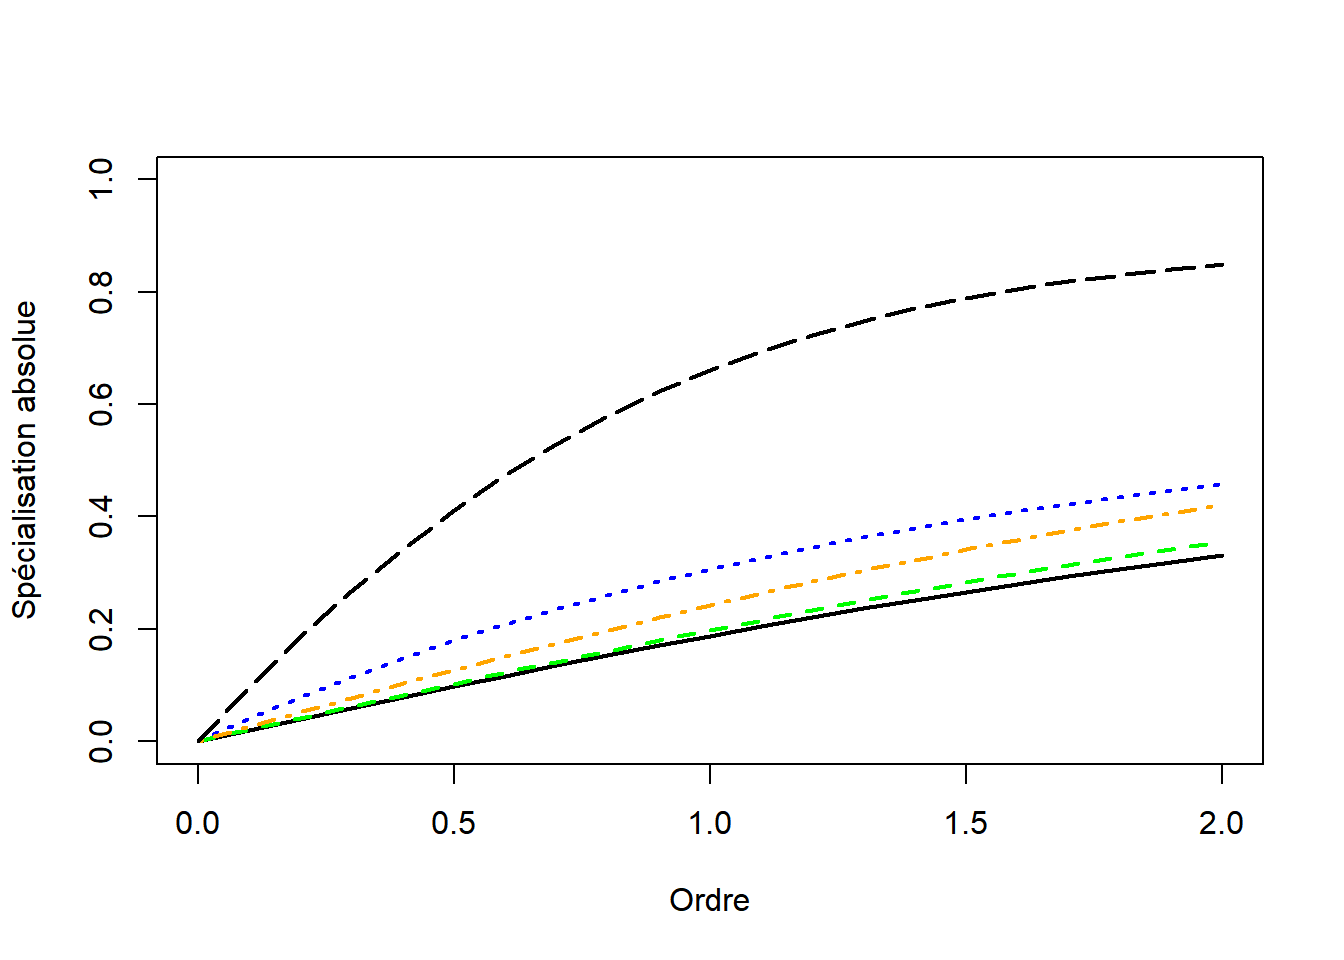
\includegraphics{Entropie_files/figure-latex/s-1.pdf}
\caption{\label{fig:s}Profils de spécialisation absolue de l'Europe (courbe
pleine, noire), de l'Italie (pointillés longs, verts), de la France
(pointillés alternés, orange), de l'Allemagne (pointillés courts, bleus)
et de l'Islande (pointillés très longs, noirs).}
\end{figure}

La diversité peut être transformée en spécialisation absolue, comme
l'ubiquité l'a été en concentration, pour obtenir la figure \ref{fig:s}.

Enfin, la spécialisation relative est le rapport entre la diversité
absolue de l'Europe entière et celle de chaque pays, visible sur la
figure \ref{fig:d}. L'Islande est le pays le plus spécialisé
relativement, avec une valeur à l'ordre 2 de 3.5 pays effectifs.

\subsection{Tests de significativité}\label{tests-de-significativite}

Deux approches sont envisageables pour tester les profils de
concentration ou spécialisation. Pour fixer les idées et sans perte de
généralité, il s'agit ici de tester la spécialisation de l'Italie contre
l'hypothèse nulle qu'elle ne serait pas différente de celle de l'Europe
entière.

La première formalisation de l'hypothèse nulle est que la distribution
des secteurs industriels en Italie est la même que celle de l'Europe
entière. Le test porte alors sur la valeur de la divergence de
Kullback-Leibler généralisée entre la distribution des secteurs en
Italie et la distribution des secteurs agrégée au niveau européen. C'est
l'approche, pour la concentration spatiale, d'Ellison et Glaeser:
\(G_s\) est la divergence d'ordre 2 entre la distribution du secteur
\(s\) et celle de l'ensemble de l'industrie. C'est aussi celle de
\citet{Mori2005} à l'ordre 1. Elle soufre de la non-indépendance des
entropies \(\alpha\) et \(\beta\) \citep{Jost2007}: la statistique
testée est l'entropie \(\beta\) mais sa valeur est contrainte par celles
de l'entropie \(\alpha\) pour une valeur donnée (de référence) de
l'entropie \(\gamma\). Une illustration du problème est qu'à l'ordre 0
l'entropie \(\beta\) est significativement différente de 0 alors que
tous les secteurs sont présents en Italie.

La formalisation alternative est que la spécialisation de l'Italie est
égale à celle d'un pays de même taille dont la distribution des secteurs
serait celle de l'Europe entière. La statistique testée est un nombre
effectif (la diversité absolue ou la spécialisation relative, de façon
équivalente). C'est l'approche retenue ici.

Le test est réalisé en générant aléatoirement, un grand nombre de fois,
de nouvelles données correspondant à l'hypothèse nulle, en calculant la
statistique d'intérêt. Les données sont simulées par 1000 tirages dans
une loi multinomiale dont les paramètres sont le nombre de personnes
travaillant en Italie et les probabilités des secteurs au niveau
européen. La spécialisation de chaque simulation est calculée pour les
ordres de 0 à 2, par intervalles de \(0.1\). Les quantiles correspondant
à 2.5\% et 97.5\% des spécialisation simulées constituent les limites de
l'enveloppe de confiance de la statistique sous l'hypothèse nulle, à
laquelle est comparée la spécialisation réelle.

Le détail du test est présenté en annexe. L'hypothèse nulle est acceptée
à l'ordre 0: la spécialisation de l'Italie est identique à celle de
l'Europe puisque dans les deux cas tous les secteurs sont présents. Dès
l'ordre \(0.1\), l'hypothèse nulle est rejetée : l'Italie est plus
spécialisée que l'Europe.

La variabilité de la spécialisation simulée est extrêmement faible parce
que les effectifs sont grands et que les personnes sont redistribuées
indépendamment les unes des autres par la loi multinomiale. Pour cette
raison, \citet{Mori2005}, à partir de données similaires, choisit de
tester la concentration spatiale des établissement en ignorant leurs
effectifs. Une bien meilleure hypothèse nulle est que les établissement
sont distribués aléatoirement, mais avec leur taille réelle, ce qui
augmente fortement l'incertitude sur la spécialisation simulée. Des
données individuelles sur les établissement, ou au minimum sur la
distribution de leurs tailles, sont nécessaires pour aller plus loin.
Avec les données disponibles, tous les profils présentés dans les
figures \ref{fig:uC} à \ref{fig:s} sont significativement différents les
uns des autres dès l'ordre \(0.1\).

\section{Diversité jointe}\label{diversite-jointe}

Le tableau de contingence des secteurs et des pays permet de décomposer
la diversité totale et d'en tirer plusieurs informations intéressantes.
Pour conserver les propriétés de la décomposition, la diversité et
l'ubiquité ne seront pas transformées en spécialisation et
concentration.

\citet{Cutrini2010} a appelé localisation globale l'information mutuelle
du tableau de contingence, c'est-à-dire la concentration relative des
secteurs, égale à la spécialisation relative des régions mesurés par la
divergence de Kullback-Leibler (l'indice relatif de Theil). Ce n'est
qu'une partie de l'information fournie par les données, la diversité ou
l'ubiquité \(\beta\), et cette approche n'est valide qu'à l'ordre 1. La
diversité jointe exploite toute l'information en combinant diversités ou
ubiquités \(\alpha\), \(\beta\) (formant ensemble la diversité
\(\gamma\)) et redondance.

\subsection{Diversité (spécialisation) des
pays}\label{diversite-specialisation-des-pays}

\begin{figure}
\centering
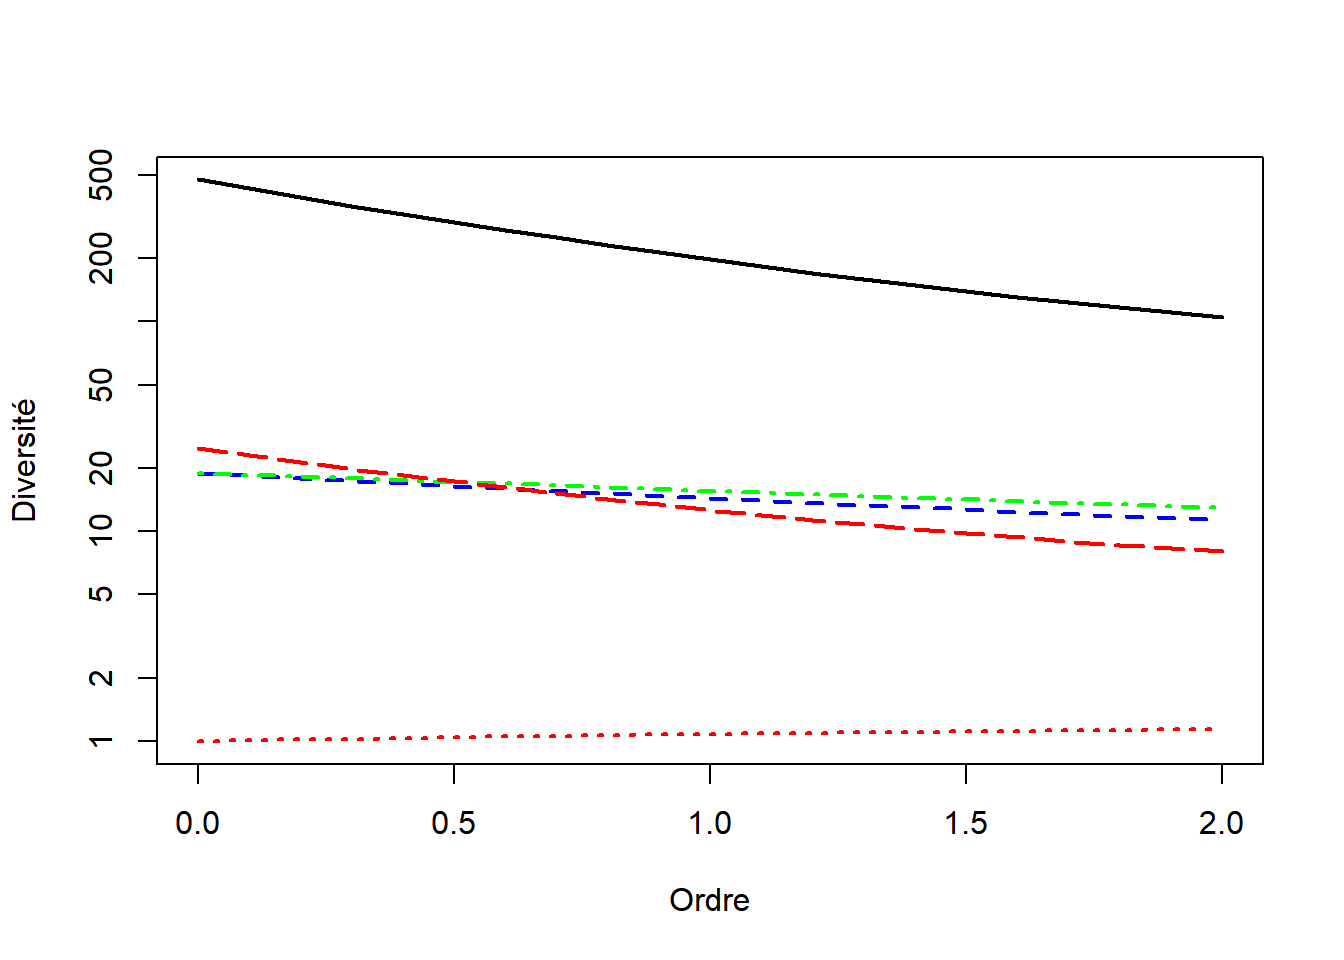
\includegraphics{Entropie_files/figure-latex/dd-1.pdf}
\caption{\label{fig:dd}Profils de diversité des pays européens: diversité
jointe (courbe pleine, noire), diversité \(\alpha\) intra-pays
(pointillés bleus), nombre effectif de pays (diversité \(\beta\),
spécialisation relative moyenne: pointillés courts, rouges), diversité
de l'Europe (\(\gamma\): pointillés longs, verts) et redondance des pays
(pointillés longs, rouges). L'échelle de la diversité est
logarithmique.}
\end{figure}

La diversité jointe est décomposée en produit de la diversité
\(\alpha\), le nombre effectif de secteurs industriels par pays, de la
diversité \(\beta\), le nombre effectif de pays, et de la redondance, le
nombre de réplications de ces pays effectifs. La diversité \(\gamma\),
produit de \(\alpha\) et \(\beta\) est celle l'Europe. La décomposition
est valide à tous les ordres de diversité, et présentée sous la forme de
profils (figure \ref{fig:dd}).

Les profils sont tracés sur une échelle logarithmique parce que les
valeurs sont d'ordres de grandeurs différents et aussi parce que la
décomposition multiplicative devient additive sous cette forme: la
hauteur de la diversité jointe sur la figure est la somme des hauteurs
des diversités \(\alpha\) et \(\beta\) et de la redondance.

La diversité de l'Europe (\(\gamma\), courbe verte) a déjà été présentée
en figure \ref{fig:cC}. Elle est très proche de la diversité \(\alpha\),
intra-pays (courbe bleue): le nombre effectif de pays (\(\beta\),
spécialisation relative, courbe rouge) varie de 1 (à l'ordre 0) à 1.1 à
l'ordre 2. Cette valeur est très faible : le maximum possible est le
nombre de pays, 25, s'ils ne partagent aucun secteur; en fait seulement
19 parce que le nombre de secteurs est ici inférieur au nombre de pays.
Les pays présentent donc un certain niveau de spécialisation absolue,
mais il est identique à celui de l'Europe entière : leur spécialisation
relative est très faible. La spécialisation relative augmente avec
l'ordre considéré, c'est-à-dire en négligeant progressivement les
secteurs de petite taille: les pays sont un peu plus différents entre
eux en ne considérant que les secteurs les plus importants.

La redondance des pays est par conséquent élevée : de 25 à l'ordre 0
(tous les pays abritent tous les secteurs) à 8 à l'ordre 2.

\subsection{Ubiquité (concentration) des
secteurs}\label{ubiquite-concentration-des-secteurs}

\begin{figure}
\centering
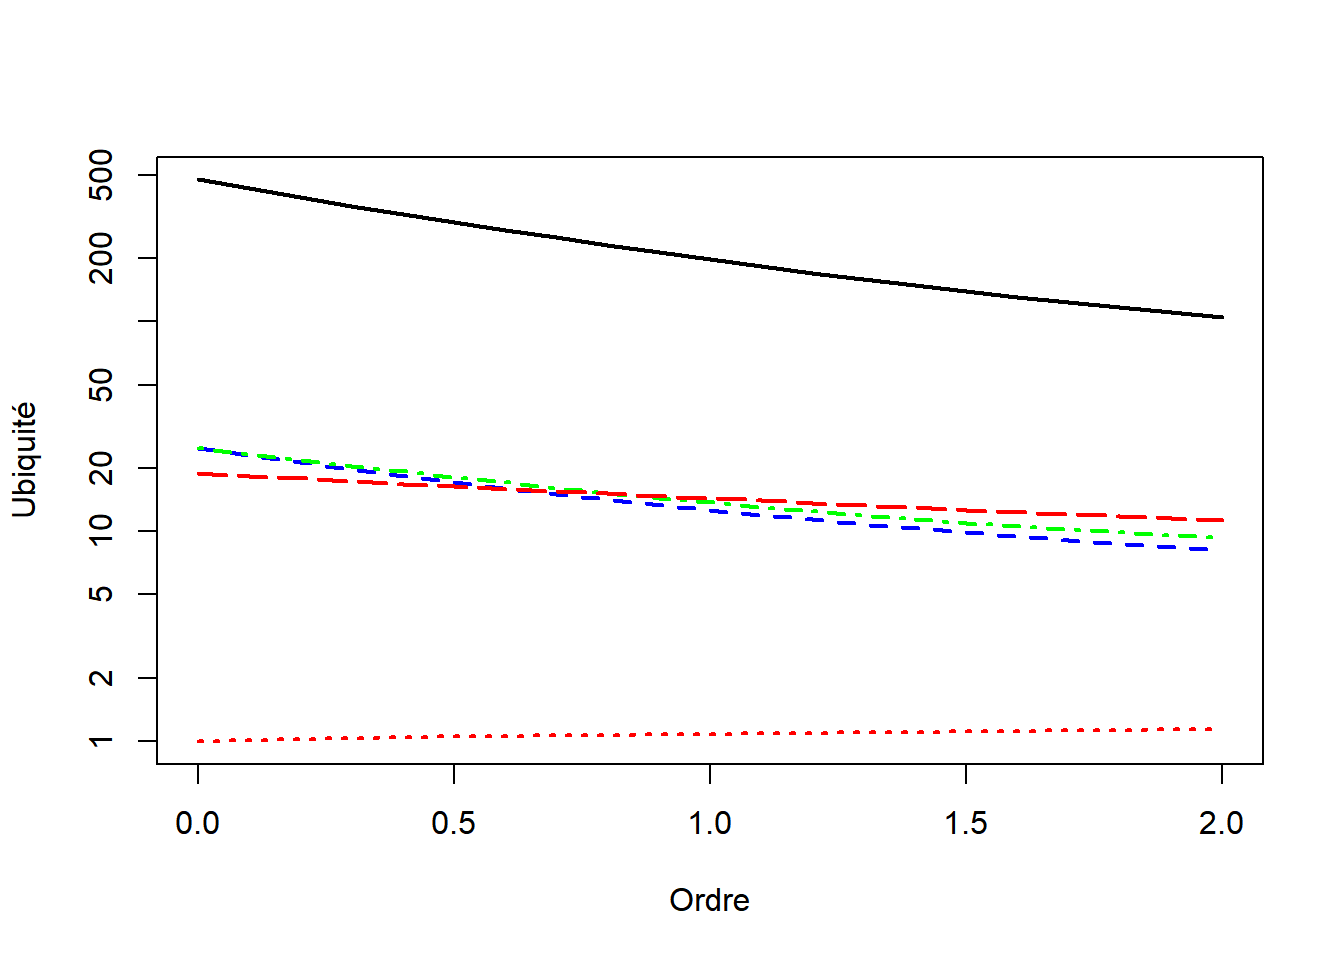
\includegraphics{Entropie_files/figure-latex/du-1.pdf}
\caption{\label{fig:du}Profils d'ubiquité des secteurs industriels:
diversité jointe (courbe pleine, noire), ubiquité \(\alpha\)
intra-sectorielle (pointillés bleus), nombre effectif de secteurs
(concentration relative, ubiquité \(\beta\): pointillés courts, rouges),
ubiquité de l'industrie entière (\(\gamma\): pointillés longs, verts) et
redondance des secteurs (pointillés longs, rouges). L'échelle est
logarithmique.}
\end{figure}

La figure \ref{fig:du} montre la décomposition de l'ubiquité des
secteurs industriels.

Les résultats sont similaires à ceux de la spécialisation. Les secteurs
sont concentrés dans l'absolu mais leur concentration relative est très
faible et la redondance est grande.

Cette grande redondance des pays et des secteurs montre qu'à ce niveau
d'agrégation des données, l'industrie européenne a une structure peu
variable entre pays ou entre secteurs.

\section{Conclusion}\label{conclusion}

La théorie de l'information, la physique statistique et l'écologie
statistique ont développé des méthodes permettant de définir et mesurer
rigoureusement l'incertitude, la diversité, et l'hétérogénéité en
général. Les méthodes qui ont été présentées ici permettent d'unifier et
d'étendre des approches répandues en économie: la mesure de la
concentration spatiale et de la spécialisation par l'entropie, et sa
décomposition. Les apports principaux sont un cadre mathématique plus
clair, l'utilisation systématique de l'entropie généralisée et la
quantification de l'hétérogénéité par des nombres effectifs qui
permettent d'interpréter clairement les grandeurs considérées.

Toutes les possibilités méthodologiques n'ont pas été explorées. Un
aspect important de la mesure de la biodiversité est son estimation à
partir de données échantillonnées plutôt que de données exhaustives
\citep{Marcon2015a}, ouvrant la possibilité d'évaluer la concentration
ou la spécialisation partir d'enquêtes plutôt que de bases de données
publiques ou commerciales. La diversité fonctionnelle ou phylogénétique
\citep{Marcon2014b} permettrait aussi de prendre en compte la
différentiation des secteurs entre eux dans l'évaluation de la
spécialisation ou la proximité des régions occupées dans la mesure de la
concentration spatiale.

%----------------------------------------------------------------------------------------
%	REFERENCE LIST
%----------------------------------------------------------------------------------------

\bibliographystyle{mee}
\bibliography{../library}

%----------------------------------------------------------------------------------------

\end{document}
